\chapter{Einleitung}
Cloud Computing hat sich in den letzten Jahren zu einem zentralen Bestandteil moderner IT-Infrastrukturen entwickelt. Unternehmen nutzen Cloud-Dienste, um ihre Anwendungen effizienter zu betreiben, Kosten zu senken und die Skalierbarkeit zu verbessern. 

Im Rahmen der Vorlesung haben wir das Themenfeld erkundet und uns mit den Möglichkeiten und Herausforderungen von Cloud Computing auseinandergesetzt. Um diese selbst auszuprobieren, haben wir die Chance, ein eigenes Projekt unter anwendung der Möglichkeiten des Coud Computing zu realisieren.

In diesem Projekt wurde eine Webanwendung unter Nutzung von Cloud Computing Ansätzen entwickelt, die dem Nutzer erlaubt von IP Adressen auf die ungefähre geographische Lage zu schließen.

\chapter{Theorie}
\section{Was ist Cloud Computing?}
Klassische IT-Infrastrukturen basieren auf physischen Servern und Rechenzentren, die vor Ort betrieben werden. Da diese jedoch oft teuer zu betreiben und schwer zu skalieren sind, setzen viele Unternehmen auf Cloud Computing.

Cloud Computing bezeichnet die Bereitstellung von IT-Ressourcen wie Servern, Speicher, Datenbanken, Netzwerken und Software über das Internet. Es gibt drei Hauptmodelle\cite{mell2011nist,hurwitz2010cloud,zhang2010towards}:
\begin{itemize}
    \item \textbf{Infrastructure as a Service (IaaS):} Bereitstellung von virtuellen Maschinen, Netzwerken und Speicher. Der Nutzer verwaltet die Infrastruktur selbst. Beispiele: AWS EC2, Azure Virtual Machines.
    \item \textbf{Platform as a Service (PaaS):} Bereitstellung einer Plattform für die Entwicklung und Bereitstellung von Anwendungen. Der Anbieter verwaltet die Infrastruktur, während der Nutzer sich auf die Anwendung konzentriert. Beispiele: Azure App Service, Google App Engine.
    \item \textbf{Software as a Service (SaaS):} Bereitstellung von Software über das Internet. Der Nutzer verwendet die Software, ohne sich um die Infrastruktur oder Plattform kümmern zu müssen. Beispiele: Google Workspace, Microsoft Office 365.
\end{itemize}

\begin{figure}[H]
    \centering
    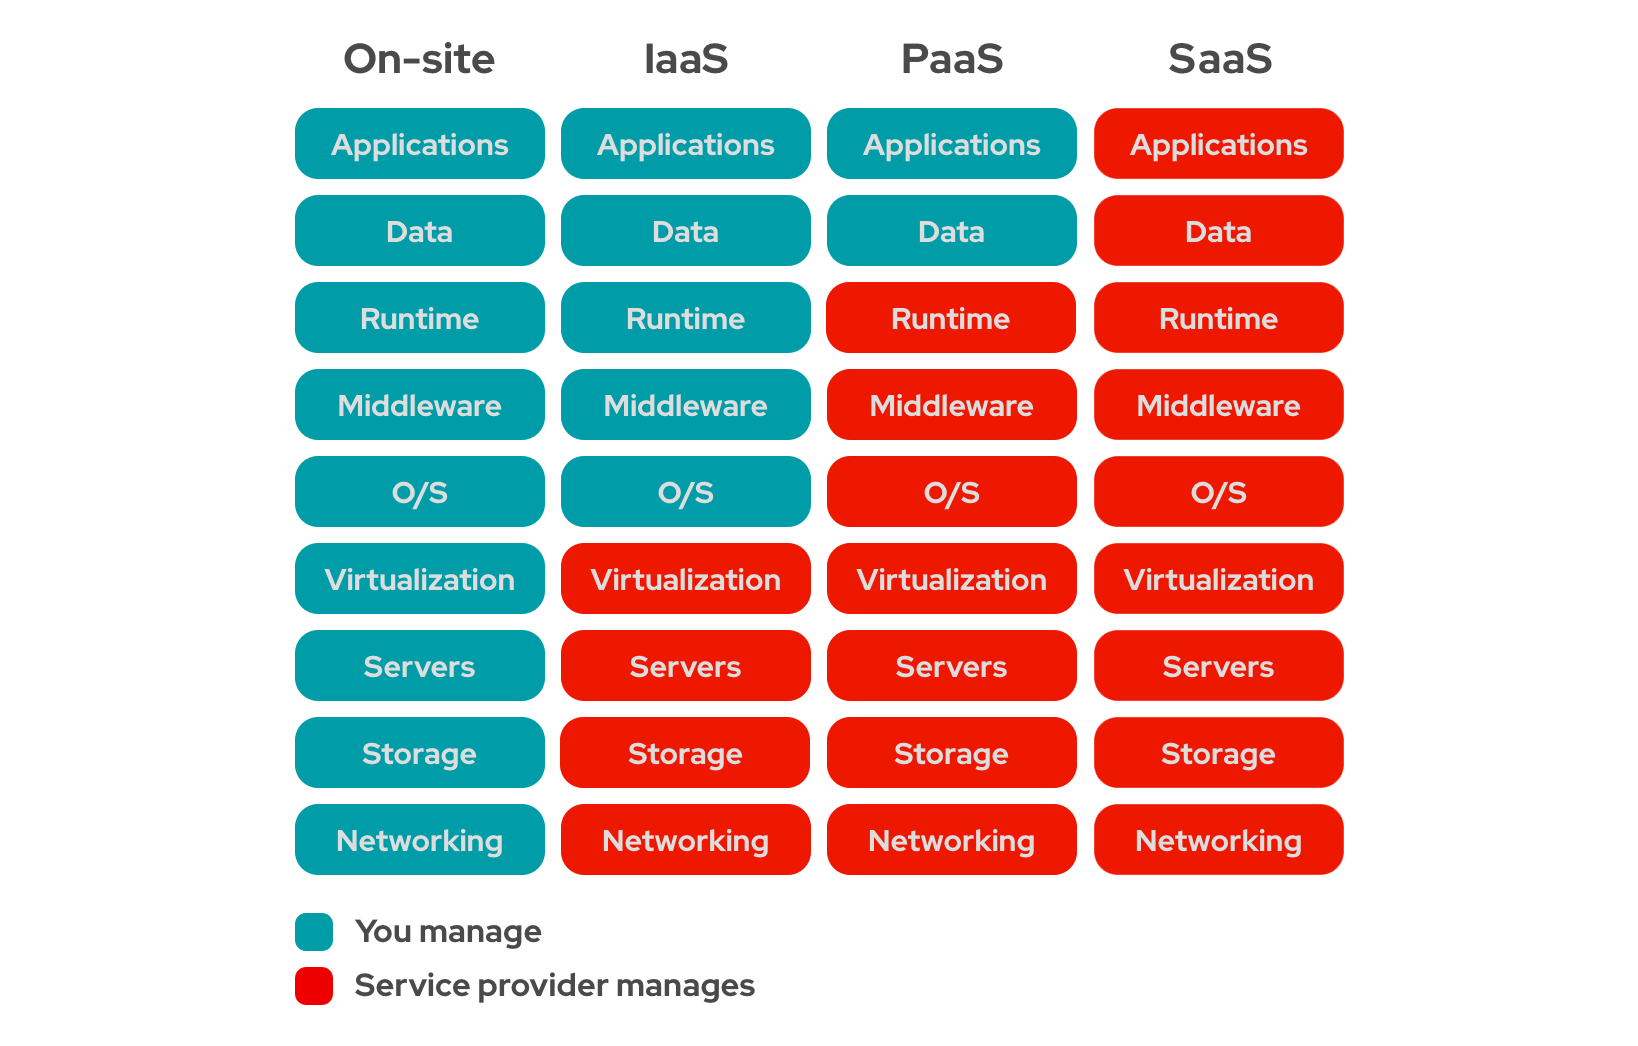
\includegraphics[width=0.8\textwidth]{resources/images/cloudcomputingtiers.png}
    \caption{Cloud Computing Modelle}
\end{figure}

\section{Warum Cloud Computing?}
Die Cloud bietet zahlreiche Vorteile:
\begin{itemize}
    \item \textbf{Skalierbarkeit:} Ressourcen können je nach Bedarf dynamisch angepasst werden.
    \item \textbf{Kostenersparnis:} Keine Investitionen in physische Hardware, Bezahlung nach Nutzung.
    \item \textbf{Flexibilität:} Zugriff auf Ressourcen von überall und jederzeit.
    \item \textbf{Automatisierung:} Tools wie Terraform und Ansible ermöglichen die einfache Verwaltung und Bereitstellung von Infrastruktur.
\end{itemize}\cite{ProCloud}

Jedoch gibt es Nachteile bei der Nutzung von Cloud Computing:
\begin{itemize}
    \item \textbf{Abhängigkeit:} Unternehmen sind von Cloud-Anbietern abhängig.
    \item \textbf{Sicherheit:} Schutz sensibler Daten und Zugriffskontrolle sind kritisch.
    \item \textbf{Kosten:} Fehlende Kontrolle über die Ressourcennutzung kann zu hohen Kosten führen.
\end{itemize}
\cite{CloudcomputingCarticle}

\section{Terraform}
Terraform ist ein Open-Source-Tool zur Infrastrukturautomatisierung. Es ermöglicht die deklarative Beschreibung von Infrastruktur als Code (IaC). Mit Terraform können Ressourcen wie virtuelle Maschinen, Netzwerke und Datenbanken in verschiedenen Cloud-Anbietern wie AWS, Azure oder Google Cloud bereitgestellt werden\cite{TerraformDocs}.

Vorteile von Terraform:
\begin{itemize}
    \item Plattformunabhängigkeit.
    \item Wiederholbare und konsistente Bereitstellung.
    \item Versionskontrolle der Infrastruktur.
\end{itemize}

\section{Ansible}
Ansible ist ein Open-Source-Tool zur Konfigurationsverwaltung und Automatisierung. Es wird verwendet, um Software zu installieren, Konfigurationen zu ändern und Anwendungen bereitzustellen\cite{AnsibleDocs}.

Folgende Features machen Ansible attraktiv:
\begin{itemize}
    \item Agentenlos: Es benötigt keine zusätzliche Software auf den Zielsystemen.
    \item Einfachheit: Konfigurationen werden in YAML geschrieben.
    \item Skalierbarkeit: Kann große Umgebungen effizient verwalten.
\end{itemize}